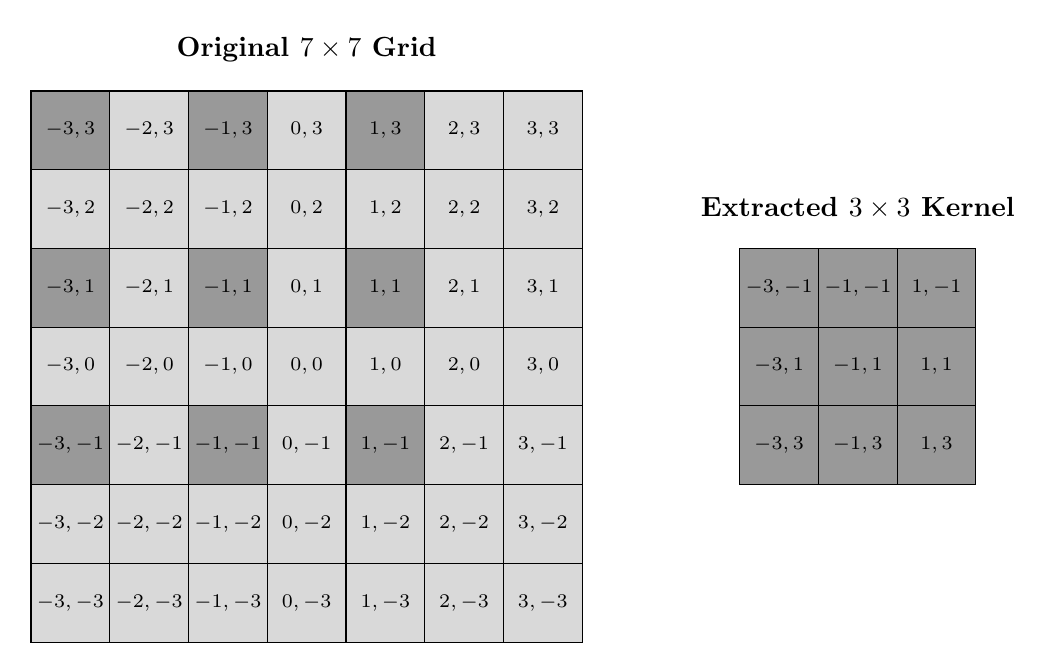
\begin{tikzpicture}
    \foreach \x in {-3,-2,-1,0,1,2,3} {
        \foreach \y in {-3,-2,-1,0,1,2,3} {
            \fill[gray!30] (\x, \y) rectangle (\x+1, \y+1);
            \draw[black] (\x, \y) rectangle (\x+1, \y+1);
        }
    }

    \fill[gray!80] (-3, 3) rectangle (-2, 4);
    \fill[gray!80] (-1, 3) rectangle (0, 4);
    \fill[gray!80] (1, 3) rectangle (2, 4);
    \fill[gray!80] (-3, 1) rectangle (-2, 2);
    \fill[gray!80] (-1, 1) rectangle (0, 2);
    \fill[gray!80] (1, 1) rectangle (2, 2);
    \fill[gray!80] (-3, -1) rectangle (-2, 0);
    \fill[gray!80] (-1, -1) rectangle (0, 0);
    \fill[gray!80] (1, -1) rectangle (2, 0);
    \draw[black] (-3, 3) rectangle (-2, 4);
    \draw[black] (-1, 3) rectangle (0, 4);
    \draw[black] (1, 3) rectangle (2, 4);
    \draw[black] (-3, 1) rectangle (-2, 2);
    \draw[black] (-1, 1) rectangle (0, 2);
    \draw[black] (1, 1) rectangle (2, 2);
    \draw[black] (-3, -1) rectangle (-2, 0);
    \draw[black] (-1, -1) rectangle (0, 0);
    \draw[black] (1, -1) rectangle (2, 0);

    \foreach \x in {-3,-2,-1,0,1,2,3} {
        \foreach \y in {-3,-2,-1,0,1,2,3} {
            \node[font=\scriptsize] at (\x+0.5, \y+0.5) {\scriptsize $\x,\y$};
        }
    }

    \foreach \i [count=\ix from -1] in {-3,-1,1} {
        \foreach \j [count=\jx from -1] in {3,1,-1} {
            \fill[gray!80] (7+\ix, \jx) rectangle (8+\ix, \jx+1);
            \draw[black] (7+\ix, \jx) rectangle (8+\ix, \jx+1);
            \node[font=\scriptsize] at (7.5+\ix, \jx+0.5) {\scriptsize $\i,\j$};
        }
    }

    \node[above] at (0.5, 4.25) {\textbf{Original $7 \times 7$ Grid}};
    \node[above] at (7.5, 2.25) {\textbf{Extracted $3 \times 3$ Kernel}};
\end{tikzpicture}
